%!TEX root=../main.tex
\chapter{User and System Testing}

\section{Contineous Usability Testing}

\subsection{Admin Interface Assessment}
Some system administrators were also asked to assess the usability of the improved admin interface. The admin interface usability assessment was not a part of the user test, as the user test focused on testing the frontend interface used by normal users. We also have an restrictive amount of system administrators which has been trained in how to use the interface, which makes a test of the admin interface on a wast amount of participants unnecessary.


\subsection{Validity}
\paragraph*{Admin Interface Assessment} \hfill \\
The number of admin users are small and might not be statistically significant. However, since the number of admin users is small and will stay small for some time in the future, it is important that the few admin users we have like the new admin interface improvements. Consequently, the assessment will likely be affected with experience from and observations done in the old admin interface. To improve the credability of the results one could also include testing of the admin interface in the optimal user test described above. However, this would make the user test more extensive and harder to execute, and would require a lot of administrative work.

\section{User Testing}
\label{sec:user-testing}

\subsection{Motivation}
A user test was performed in the In-Depth study delivered in December 2015 as mentioned in sub-section \ref{subsec:related-proj}. The \gls{cmb} system was one of three tools used by the students in mandatory assignments, where the \gls{cmb} system mainly was used for testing the system on more users then previously attempted by Follan and Støa \cite{mt:T&S}. The course assignments cover various topics and methods of producing parallel code in C++, like OpenMP, NEON, MPI and CUDA, and is about 25\% of the workload during the semester for the avarage student. The TDT4200 course staff added in total 5 programming problems to \gls{cmb} which were solvable by students, and the system received a lot of submissions during the semester. During November of 2015, a total of 37 students delivered a optional questionnaire which included some questions about the \gls{cmb} system. In addition to the questionnaire, some feedback on the system was gathered during the last lecture of the course. The feedback were mainly focused on usability aspects of the system, which helped the \gls{cmb} project team to discover bugs and to setup and prioritize features to implement next. These were presented in the backlog found in the In-Depth study project report. \\

\subsection{Methodology}
The user test conducted April 18th this Spring assesses the system improvements presented in Chapter \ref{ch:improvements} with focus on usability. The goal of the test is to further improve the results from the TDT4200 questionnaire. The test required an interest in programming and programming experience from the participants, but no prior knowledge of C or C++ or any parallel programming libraries offered by the system were set as a requirement. The weak requirements were set since there were generally little interest from students in participating in the test, most likely due to bad timing. Most students have several assignment deliverables before the last lecture in mid April. Further, attracting students or others to participate in user tests for a master thesis is generally hard. \textit{As the focus of this test were to test the usability of the system, it should be sufficient for participants to have general knowledge and interest in programming to assess if the system is usable or not}. The user test described a set of tasks to be completed by each participant, and Appendix \ref{apdx:usertest} presents the tasks along with a questionnaire each participant were to complete before finishing the user test. Nearly all participants conducted the test simultanously in a lecture hall to simulate the heavy submission traffic we experienced before assignment deadlines in TDT4200. A couple of participants started the user test late or participated a couple of days after the official user test, to simulate the students in TDT4200 that experienced little or no traffic. Participants were informed that questions related to how to complete a task would not be answered during the test and that tasks should be completed individually. They were also informed that they could abort the test at any time. \\

\begin{table}
    \centering
    \begin{tabular}{ | l | p{6cm} |}
    \hline
    \textbf{Problem Name} & \textbf{Problem Description Summary} \\ \hline
    Hello World & Print out "Hello World!"". \\ \hline
    Digits & \textit{T} test cases are given as input, each test case describing the range between two numbers \textit{N} and \textit{M}. For each test case, output the number of zeroes present in all the numbers in the range [\textit{N}, \textit{M}]. \\ \hline
    Prime Number & For every number in the input, output if the number is a prime. \\ \hline
    WERTYU & For every encrypted input string, decrypt it and output the decrypted string. Hint: The input strings are encrypted with an QWERTY keyboard shifted one character to the right. \\ \hline
    Reverse String & For every input string output the reversed string. \\
    \hline
    \end{tabular}
    \caption{Available Solvable Problems During User Test}
    \label{tab:avail-prob}
\end{table}

The most time consuming task the participants had to complete were to submit code to one of the problems presented in Table \ref{tab:avail-prob}. Submitting code to problems is the core of the \gls{oj} and the process of uploading and running submissions were the most common procedure done by TDT4200 students. The procedure and aspects related to submissions was also mentioned the most times in the comments by the TDT4200 students, and was therefore chosen as one of the main tasks to perform in this user test. Before starting the user test, the participants were also notified to comment extensively on the procure when filling out the survey. The participants who were unfamiliar with C and C++ were given 5 different source files to the "Prime Number"-problem which they were to submit to the system, to simulate that the participants made a number of tries before arriving at the correct solution. The problem were chosen as it is of medium to easy difficulty. Participants who knew either C or C++ were also motivated to try to solve more than one problem if they arrived at a solution quickly, to extensively test the procedure of uploading and running submissions. Other tasks executed by participants included sign-up, login, viewing submissions and highscore lists, joining groups, creating and administering groups, and changing user e-mail and password. \\

The questionnaire found in Appendix \ref{apdx:usertest} contains the same questions about the \gls{cmb} system presented in the questionnaire given to the students in TDT4200. In addition, a couple of extra questions were added for the sake of clarity. It is important that the questionairre matches to be able to compare the results of the two tests. The questionnaire builds upon a combination of the Likert scale multiple choice questions and textual based questions. Likert scale is well known when it comes to measuring the usability of software systems and in this test the number of alternatives per question is set to five. Each row in Table \ref{tab:likert-scale} shows the possible alternatives for a given question. Furthermore, the textual based questions are added to make it easier for the participants to describe their thoughts about aspects of the system in great detail. \\

\begin{table}[t!]
    \centering
    \begin{tabular}{ | c | p{1.6cm} | p{1.6cm} | p{1.6cm} | p{1.6cm} | p{1.6cm} |}
    \hline
    \textbf{Question Type} & \multicolumn{5}{ c| }{\textbf{Likert Range}} \\ \hline
    1 & Very poor & Poor & Neutral & Good & Very good \\ \hline
    2 & Strongly disagree & Disagree & Neither agree or disagree & Agree & Strongly agree \\ \hline
    3 & Very hard & Hard & Neutral & Easy & Very easy \\ \hline
    4 & Not satisfied at all & A little bit satisfied & Neutral & Satisfied & Very satisfied \\ \hline
    \end{tabular}
    \caption{Likert Scale Alternatives on Question Type}
    \label{tab:likert-scale}
\end{table}

\subsection{Results and Evaluation}

\begin{figure}
    \centering
    %\hspace*{-1.5cm}
    \begin{subfigure}[h]{0.48\textwidth}
        \centerline{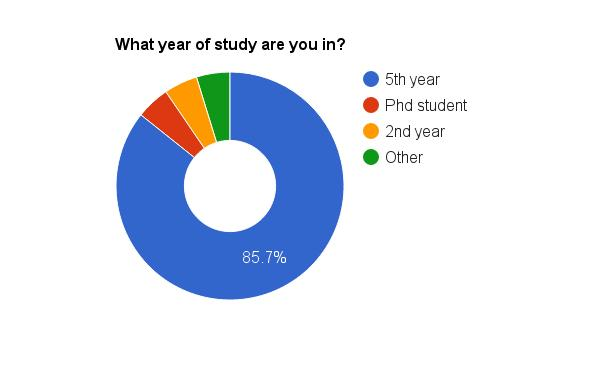
\includegraphics[width=1.5\textwidth]{results/year_of_study.jpg}}
        \caption{}
        \label{fig:year-of-study}
    \end{subfigure}
    ~ %add desired spacing between images, e. g. ~, \quad, \qquad, \hfill etc.
      %(or a blank line to force the subfigure onto a new line)
    \hfill
    \begin{subfigure}[h]{0.48\textwidth}
        \centerline{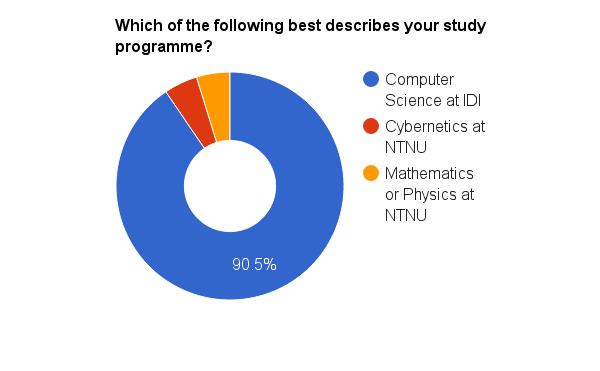
\includegraphics[width=1.5\textwidth]{results/study_programme.jpg}}
        \caption{}
        \label{fig:study-programme}
    \end{subfigure}
    %add desired spacing between images, e. g. ~, \quad, \qquad, \hfill etc.
    %(or a blank line to force the subfigure onto a new line)

    %\hspace*{-1.5cm}
    \begin{subfigure}[h]{0.48\textwidth}
        \centerline{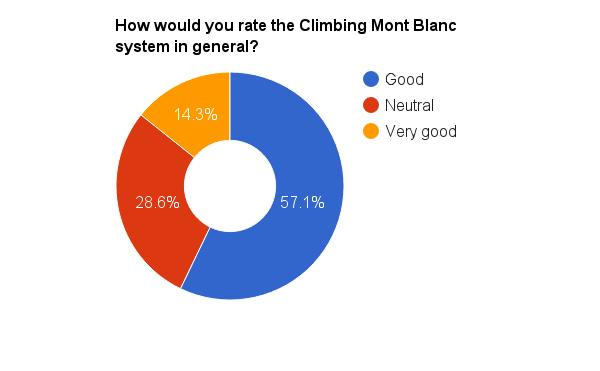
\includegraphics[width=1.5\textwidth]{results/general_cmb.jpg}}
        \caption{}
        \label{fig:cmb-general}
    \end{subfigure}
    \hfill
    \begin{subfigure}[h]{0.48\textwidth}
        \centerline{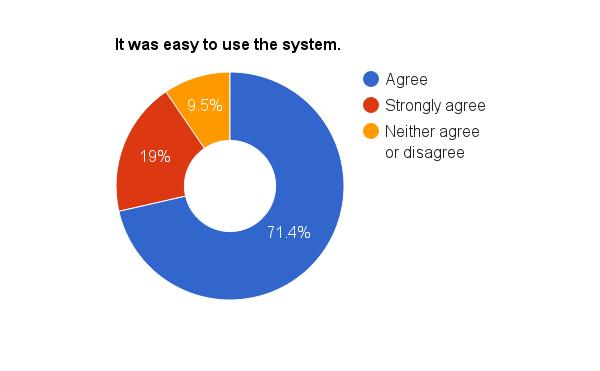
\includegraphics[width=1.5\textwidth]{results/easy_to_use.jpg}}
        \caption{}
        \label{fig:cmb-easy-use}
    \end{subfigure}
    \caption{Multiple Choice Results}
    \label{fig:multiplechoice}
\end{figure}


\begin{figure}
    \centering
    %\hspace*{-1.5cm}
    \begin{subfigure}[h]{0.48\textwidth}
        \centerline{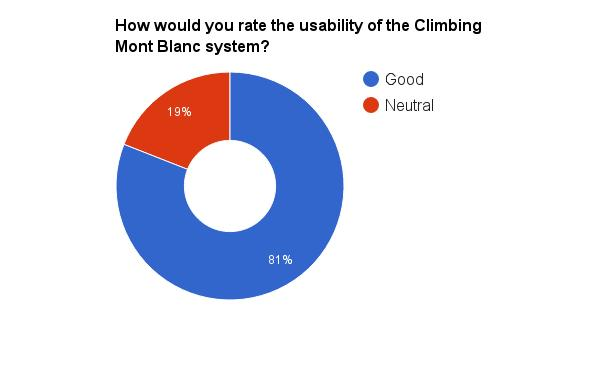
\includegraphics[width=1.5\textwidth]{results/usability_cmb.jpg}}
        \caption{}
        \label{fig:cmb-usability}
    \end{subfigure}
    ~ %add desired spacing between images, e. g. ~, \quad, \qquad, \hfill etc.
      %(or a blank line to force the subfigure onto a new line)
    \hfill
    \begin{subfigure}[h]{0.48\textwidth}
        \centerline{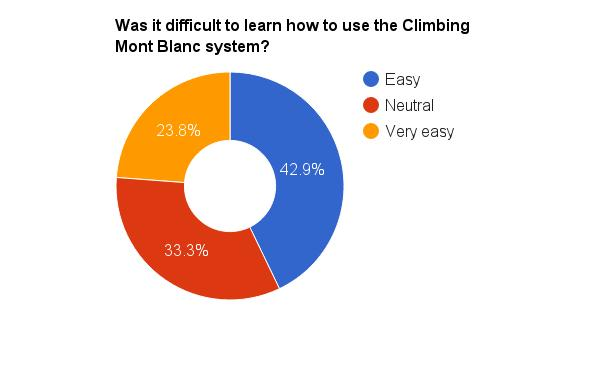
\includegraphics[width=1.5\textwidth]{results/learn_cmb.jpg}}
        \caption{}
        \label{fig:cmb-learn}
    \end{subfigure}

    %\hspace*{-1.5cm}
    \begin{subfigure}[h]{0.48\textwidth}
        \centerline{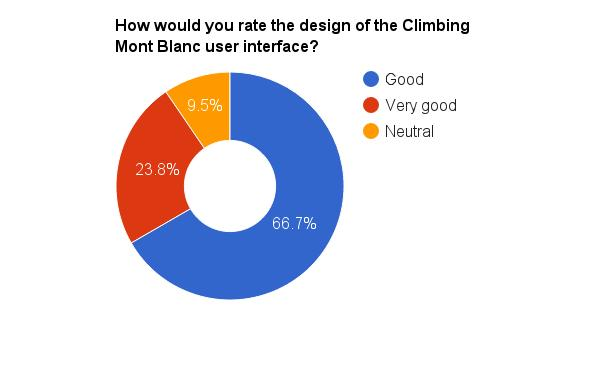
\includegraphics[width=1.5\textwidth]{results/design_cmb.jpg}}
        \caption{}
        \label{fig:cmb-design}
    \end{subfigure}
    ~ %add desired spacing between images, e. g. ~, \quad, \qquad, \hfill etc.
      %(or a blank line to force the subfigure onto a new line)
    \hfill
    \begin{subfigure}[h]{0.48\textwidth}
        \centerline{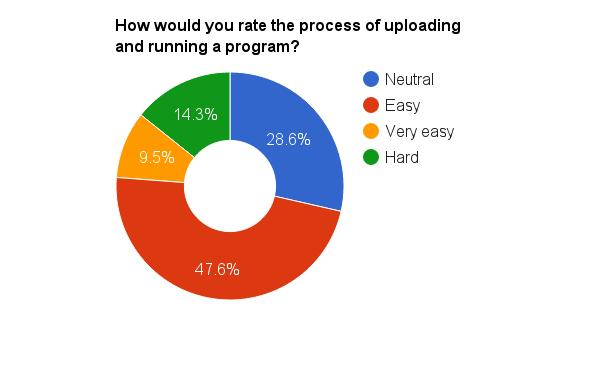
\includegraphics[width=1.5\textwidth]{results/submission_cmb.jpg}}
        \caption{}
        \label{fig:cmb-submission}
    \end{subfigure}
    \caption{Multiple Choice Results (continuation of Figure \ref{fig:multiplechoice})}
    \label{fig:multiplechoice1}
\end{figure}

\begin{figure}
    \centering
    %\hspace*{-1.5cm}
    \begin{subfigure}[h]{0.48\textwidth}
        \centerline{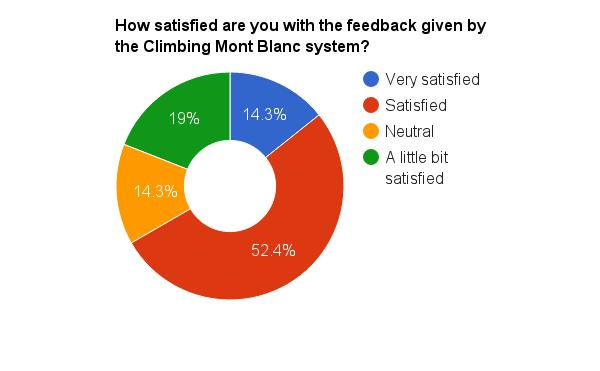
\includegraphics[width=1.5\textwidth]{results/feedback_cmb.jpg}}
        \caption{}
        \label{fig:cmb-feedback}
    \end{subfigure}
    \hfill
    \begin{subfigure}[h]{0.48\textwidth}
        \centerline{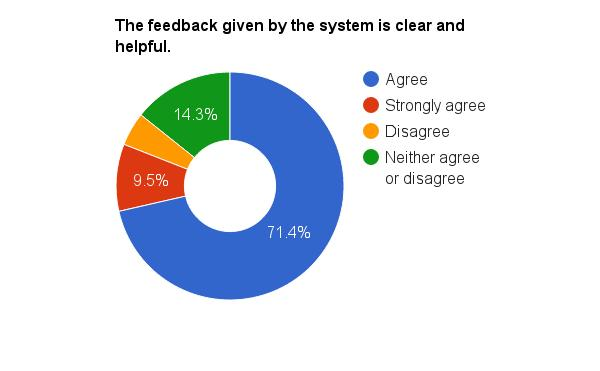
\includegraphics[width=1.5\textwidth]{results/clear_feedback_cmb.jpg}}
        \caption{}
        \label{fig:cmb-feedback-clear}
    \end{subfigure}

    %\hspace*{-1.5cm}
    \begin{subfigure}[h]{0.48\textwidth}
        \centerline{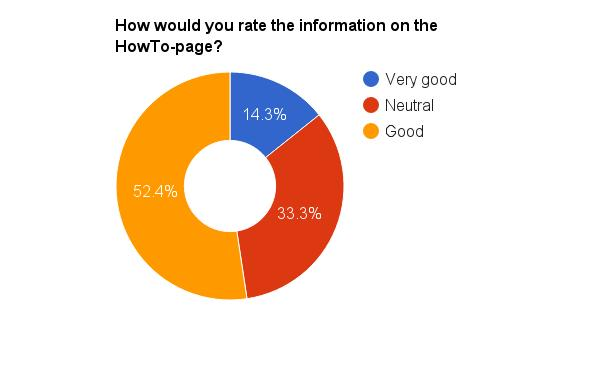
\includegraphics[width=1.5\textwidth]{results/howto_cmb.jpg}}
        \caption{}
        \label{fig:cmb-howto}
    \end{subfigure}
    \caption{Multiple Choice Results (continuation of Figure \ref{fig:multiplechoice1})}
    \label{fig:multiplechoice2}
\end{figure}

There were in total 21 participants in the user test. The Figures \ref{fig:multiplechoice}, \ref{fig:multiplechoice1}, \ref{fig:multiplechoice2} shows the results of the multiplechoice questions.


A total of 37 TDT4200 students provided feedback in the optional questionnaire given during the Autmumn semester, and the reader is noted about that the statistical difference might weaken the conclusions made here.

\subsection{Threats to Validity}
\paragraph*{User Test} \hfill \\
There are multiple factors in the experimental setup and execution of this test that may threaten the internal validity of the results. First, the participants in the user test does not necessarily have the same background and interests as the students in the course TDT4200. This may have an effect on how the participants percieve the system, and it may be different from the perception made by students students in TDT4200. Most of the TDT4200 students are interested in low-level and parallel programming, and may have little interest in design or frontend functionality as long as the system is in some way usable. A possible side effect might be that the two groups perceive the system usability differently. \\

Second, the participants of this test used the system for a short period of time. The students in TDT4200 used the system in a total of 5 exercises throughout the Autumn semester, and have tried using the system multiple times. The participants in this test may not have been able to test the system thoroughly like the students in TDT4200 had a chance to do. Third, the number of participants in this test may not be as statistically significant as in the user test conducted during the Autumn. Conclusions drawn from unequal quantities of participants in the two tests may be less correct than two tests having equal amount of participants, and the reader should keep this in mind during evalution. Fourth, since it was hard to get participants to the test, many of the participants are friends of or familiar to the \gls{cmb} team. This might further affect the results in either a positive or negative way. \\

There are also a number of ways to setup user tests than the setup described above. As mentioned, it was hard to get participants to the user test and the test therefore only used the improved version of the system. Another possibility would be to split the participants into two groups, and have each group try out both the older and the improved system. One of the groups would then start out with the new system and the other group with the old, filling out a questionnaire before switching system. The downside with this method however, is that the users starting out with the old system might be affected when assessing the usability of the new system or vice versa. The test also takes double the amount of time to execute and requires more administrative work. The optimal experimental setup would be to have preferably 60-80 random people with an interest for C or C++ and parallel computing, such that the group could be split into two random groups of participants where each group either tested the old or the improved system. Comparing usability would then be more valid and conclusions drawn would probably be more correct.


\section{System Unit Tests}

\subsection{Coverage}

\subsection{Validity}
